The Vortex Æther Model (VAM) advances a multimodal conception of time, rooted in the internal and relational dynamics of an incompressible, inviscid æther. Unlike the unidimensional time parameter in standard field theory or the proper time of General Relativity, VAM’s temporal taxonomy encapsulates distinct physical, topological, and informational modes, each with a clear analytical and experimental role. This layered approach not only extends Einstein’s “geometric æther” but also provides a framework for modeling causality, memory, and quantum-classical transitions in a unified manner~\cite{VAM-8, VAM-13, VAM-15}.

The multimodal temporal ontology of VAM is not purely an abstract taxonomy; it possesses a geometric and topological structure, naturally visualized as a multidimensional “spiral” or “fan” in phase space (see Fig.~\ref{fig:temporal_ontology}). Each temporal mode—Aithēr-Time, Now-Point, Chronos-Time, Swirl Clock, Vortex Proper Time, and Kairos Moment—plays an independent yet interconnected role, governing different layers of physical law~\cite{VAM-8, VAM-13}.

\begin{figure}[htb]
    \centering
    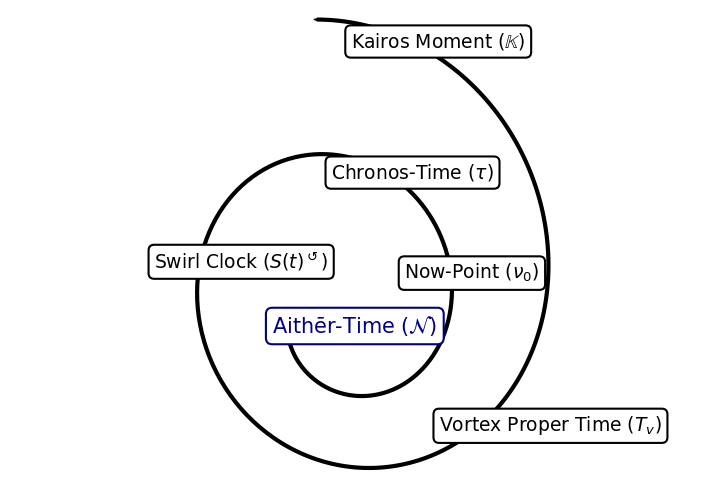
\includegraphics[width=0.7\textwidth]{TemporalOntology}
    \caption{
        \textbf{Vortex Phase Spiral of Ætheric Time.}
        The sequential emergence of time modes in the VAM ontology, proceeding outward from the core of Aithēr-Time ($\boldsymbol{\mathcal{N}}$), through Now-Point ($\boldsymbol{\nu_0}$), Chronos-Time ($\boldsymbol{\tau}$), Swirl Clock ($\boldsymbol{S}^{\boldsymbol{\circlearrowleft}}_\text{(t)}$), Vortex Proper Time ($\boldsymbol{T_v}$), to the outermost Kairos Moment ($\mathbb{\boldsymbol{K}}$). Each layer represents a distinct analytical and physical role, together forming a unified temporal architecture underlying vortex dynamics~\cite{VAM-8, VAM-13}.
    }
    \label{fig:temporal_ontology}
\end{figure}

\begin{tcolorbox}[
  colback=gray!10,
  colframe=black,
  width=1.0\textwidth,
  sharp corners=southwest,
  boxrule=0.5pt,
  before skip=10pt,
  after skip=10pt,
  title=\textbf{Table: Ætheric Time Modes in the Vortex Æther Model},
  fonttitle=\bfseries,
]
\renewcommand{\arraystretch}{1.25}
\small
\begin{tabular}{r l l}
  $\boldsymbol{\mathcal{N}}$     & \textbf{Aithēr-Time}         & Absolute causal ordering parameter~\cite{VAM-8, VAM-13} \\
  $\boldsymbol{\nu_0}$           & \textbf{Now-Point}           & Localized intersection with universal present~\cite{VAM-8, VAM-13} \\
  $\boldsymbol{\tau}$            & \textbf{Chronos-Time}        & Measurable time in the æther (subject to dilation)~\cite{VAM-1, VAM-8} \\
  $\boldsymbol{S}^{\boldsymbol{\circlearrowleft}}_\text{(t)}$ & \textbf{Swirl Clock}         & Internal phase memory of a vortex~\cite{VAM-2, VAM-13, VAM-15} \\
  $\boldsymbol{T_v}$             & \textbf{Vortex Proper Time}  & Circulation-based geodesic duration~\cite{VAM-2, VAM-13} \\
  $\mathbb{\boldsymbol{K}}$      & \textbf{Kairos Moment}       & Discrete topological bifurcation event~\cite{VAM-13, VAM-15} \\
\end{tabular}
\end{tcolorbox}

\noindent The interpretation of each mode is as follows:
\begin{itemize}
    \item \textbf{Aithēr-Time ($\boldsymbol{\mathcal{N}}$):} The unobservable but indispensable global time parameter that orders all events causally within the ætheric manifold, serving as the absolute temporal background for physical processes~\cite{VAM-8, VAM-13}.

    \item \textbf{Now-Point ($\boldsymbol{\nu_0}$):} The localized realization of the present, defined by the intersection of the global time field $\boldsymbol{\mathcal{N}}$ with a point in the æther manifold. It establishes the surface of simultaneity and facilitates causal foliation~\cite{VAM-8, VAM-13}.

    \item \textbf{Chronos-Time ($\boldsymbol{\tau}$):} The physically measurable flow of time, experienced within the æther and modulated by local vorticity through swirl-induced time dilation~\cite{VAM-1, VAM-8}:
    \[
        \frac{d\boldsymbol{\tau}}{dt} = \sqrt{1 - \boldsymbol{v_\phi}^2(r)/c^2}
    \]
    where $\boldsymbol{v_\phi}(r)$ is the local tangential velocity of the vortex field.

    \item \textbf{Swirl Clock ($\boldsymbol{S}^{\boldsymbol{\circlearrowleft}}_\text{(t)}$):} The internal phase variable of a vortex structure, tracking angular displacement and serving as a memory function for topological identity and history. It is formally given by~\cite{VAM-2, VAM-13}:
    \[
        \boldsymbol{S}^{\boldsymbol{\circlearrowleft}}_\text{(t)} = \int_{0}^{t} \boldsymbol{\Omega}(r(t'))\, dt'
    \]
    with $\boldsymbol{\Omega}(r)$ the local angular velocity.

    \item \textbf{Vortex Proper Time ($\boldsymbol{T_v}$):} The intrinsic circulation-based duration associated with a closed path around a vortex core, defined as~\cite{VAM-2, VAM-13}
    \[
        \boldsymbol{T_v} = \oint \frac{dl}{\boldsymbol{v_\phi}(r)}
    \]
    representing the intrinsic “clock” of a knotted structure.

    \item \textbf{Kairos Moment ($\mathbb{\boldsymbol{K}}$):}
    The discrete event marking a topological transition such as vortex reconnection or bifurcation, producing an irreversible change in vortex identity and introducing discontinuities or non-analyticities in the evolution of $\boldsymbol{T_v}$ or $\boldsymbol{S}^{\boldsymbol{\circlearrowleft}}_\text{(t)}$~\cite{VAM-13, VAM-15}.
\end{itemize}

In the VAM framework, the “Kairos Moment” ($\mathbb{\boldsymbol{K}}$) represents a discrete, topologically induced transition in the evolution of vortex matter—such as a vortex reconnection, bifurcation, or the passage of a gravitational wave. These events break the smooth evolution of the Swirl Clock phase and manifest as quantized phase slips or time jumps. As shown in Fig.~\ref{fig:kairos_moment}, a Kairos event appears as an abrupt change in the Swirl Clock trajectory during a localized temporal window. Such phenomena are experimentally accessible in analog systems and may be detectable in astrophysical settings as phase anomalies or decoherence events in quantum or classical fields~\cite{VAM-13, VAM-15}.

\begin{figure}[htb]
    \centering
    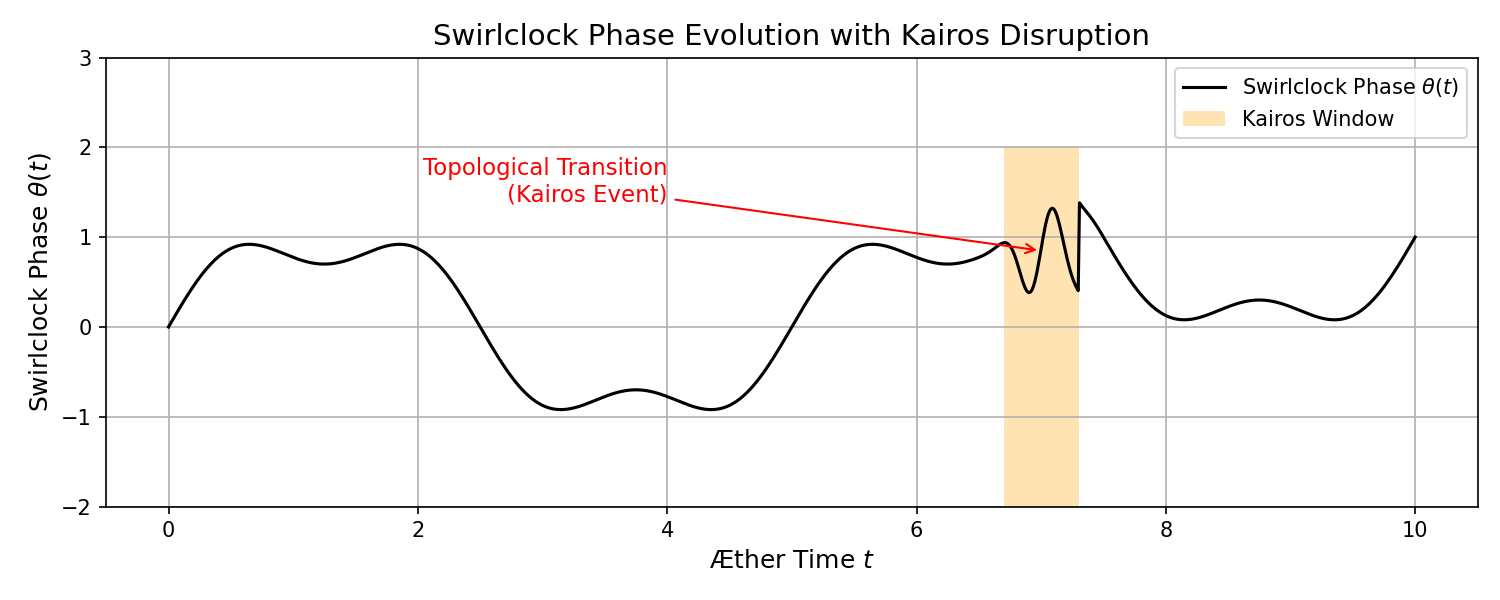
\includegraphics[width=0.7\textwidth]{TemporalOntologyKairosMoment}
    \caption{
        \textbf{Swirlclock Phase Evolution with Kairos Disruption.}
        The evolution of the Swirl Clock phase, $\theta(t)$, as a function of Æther Time ($t$), illustrating a topological transition (“Kairos Event”) as a discontinuity in the phase trajectory. The highlighted “Kairos Window” denotes the temporal interval where a critical event (such as vortex reconnection or a passing gravitational wave) induces an irreversible shift or decoherence in the internal phase. Such events correspond to the “Kairos Moment” ($\mathbb{\boldsymbol{K}}$) in the VAM temporal ontology, marking the transition from smooth, memory-preserving evolution to a new dynamical regime. This demonstrates how topological or energetic disruptions in the æther manifest as observable time “jumps” or phase slips in physical systems~\cite{VAM-13, VAM-15}.
    }
    \label{fig:kairos_moment}
\end{figure}

This multimodal temporal ontology enables VAM to bridge metaphysical continuity with physically testable vortex dynamics. It underpins several core applications in the extended VAM literature, including models of causality, gravitational time dilation, vortex identity, and swirl-induced phase decoherence~\cite{VAM-1, VAM-2, VAM-8, VAM-13, VAM-15}. For detailed derivations, see~\cite{VAM-2, VAM-8, VAM-13, VAM-15}.